\chapter{Data Processing}


\begin{figure}
	\centering
	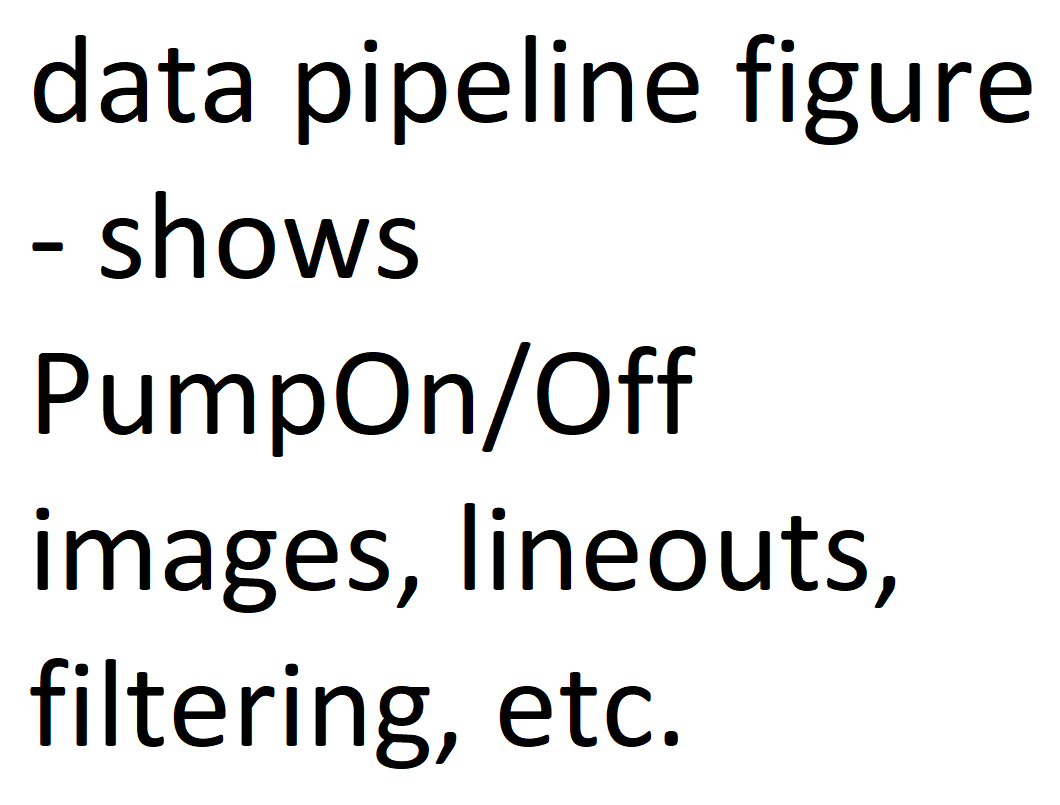
\includegraphics[width=0.5\textwidth]{figures/chap3/Data_Pipeline.png}
	\caption{this figure shows the data processing pipeline. it shows how we start with PumpOn-Off 2D images and transform them into spectrograms. it includes steps like an absorbance (A) calculation, spectral lineouts, frequency filtering and smooth, energy calibration, etc.}
	\label{fig:Data_Pipeline}
\end{figure}

\begin{figure}
	\centering
	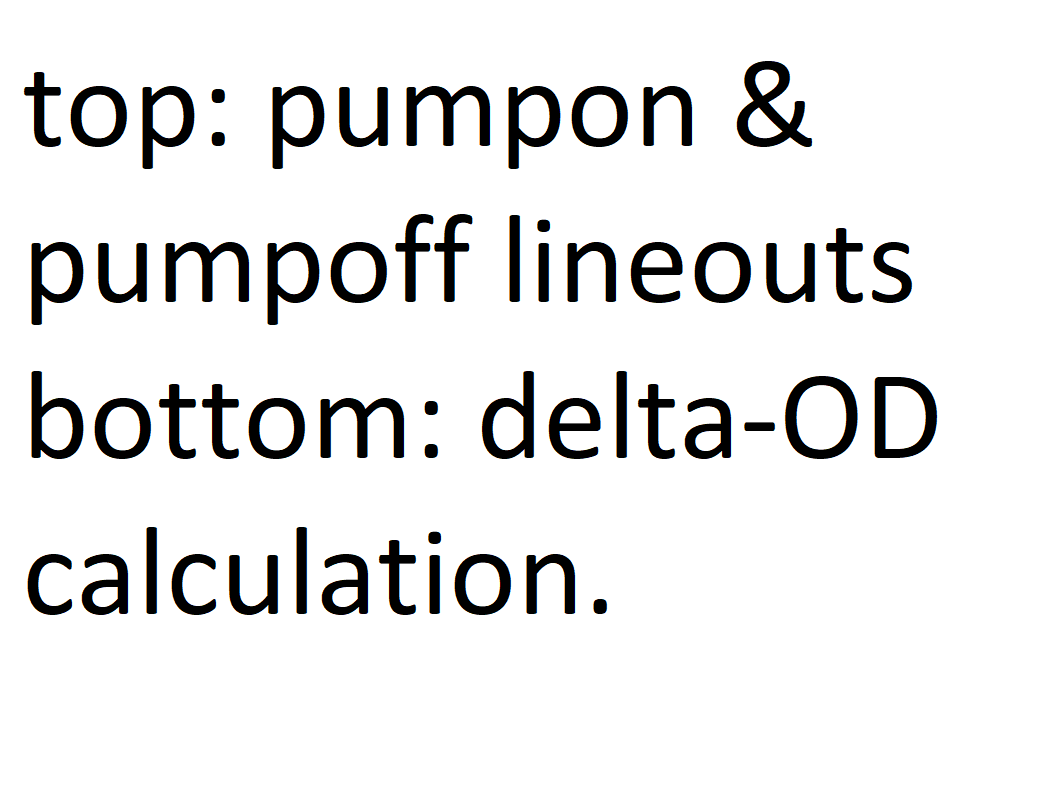
\includegraphics[width=0.5\textwidth]{figures/chap3/PumpOn_vs_PumpOff.png}
	\caption{this figure shows, using real data, a pump off and pump on spectral lineout. in another panel, it shows the $\Delta A$.}
	\label{fig:PumpOn_vs_PumpOff}
	% data set: C:\testdata\2019_09_06\52mV
	% figure made using: ???
\end{figure}

\begin{figure}
	\centering
	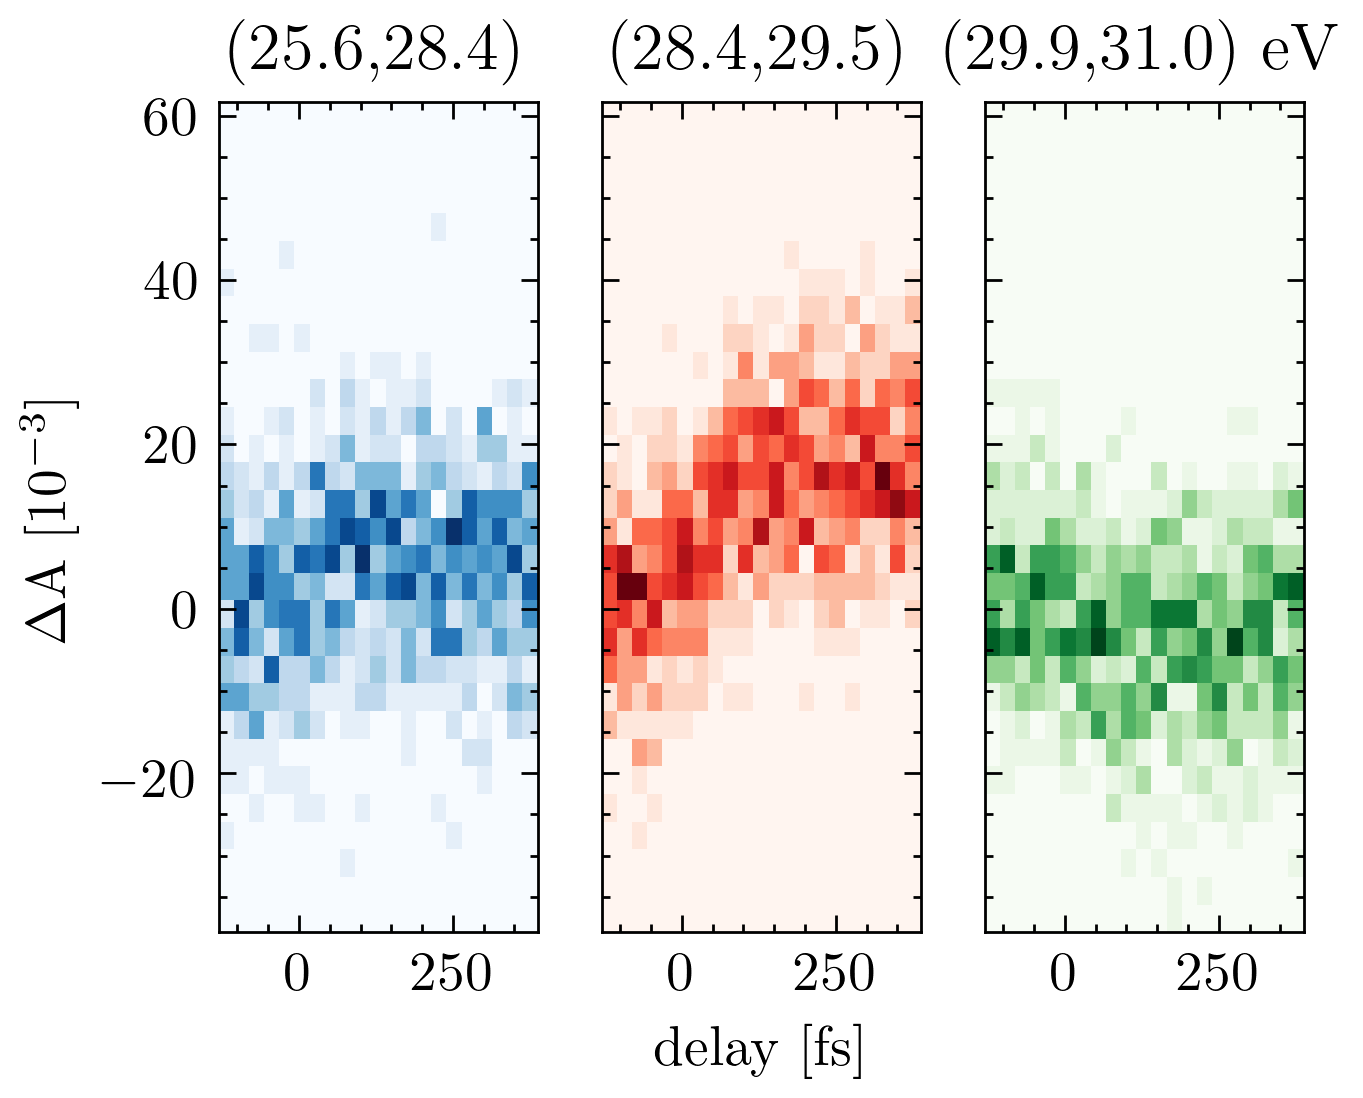
\includegraphics[width=0.5\textwidth]{figures/chap3/uncorrected_hist.png}
	\caption{$N=50$ averaged delay scans. no corrections have been made to the data. histogram of $\Delta A$ for 3 selected features. dataset is same as \cref{fig:Ge_uncorrected_raw_spectrogram}.}
	\label{fig:uncorrected_hist}
	% data set: ???
	% figure made using: ???
\end{figure}


\begin{figure}
	\centering
	\subfloat[$C(\tau,E)$]{
		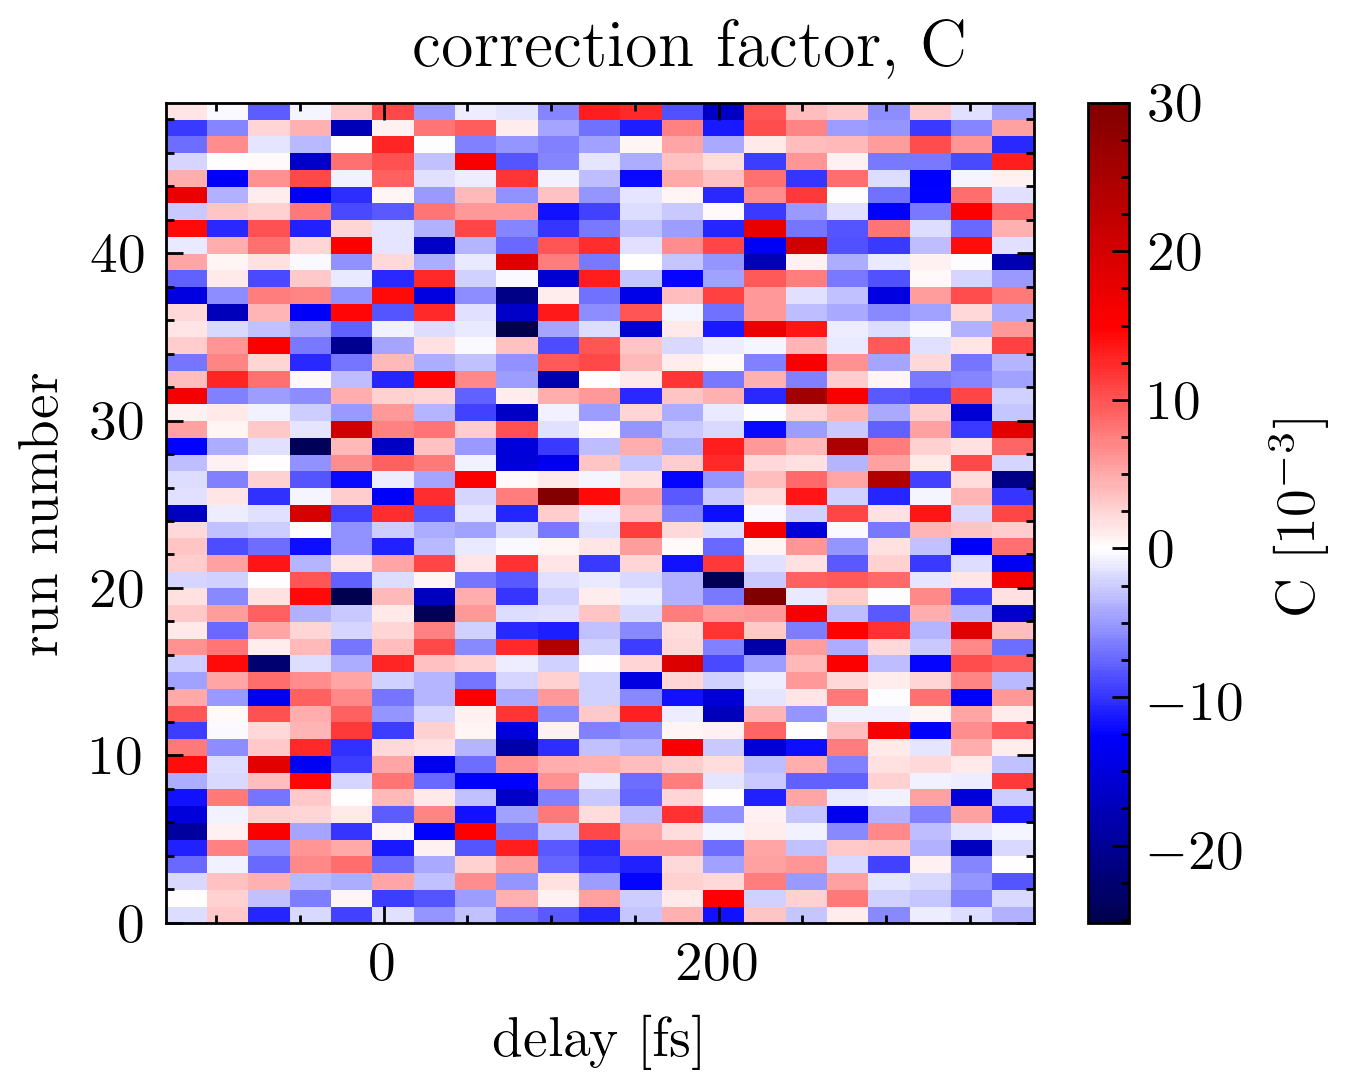
\includegraphics[width=0.4\textwidth]{figures/chap3/C_factor_image.png}
		\label{fig:C_factor_image}}
	\qquad
	\subfloat[Histogram of $C(\tau,E)$]{
		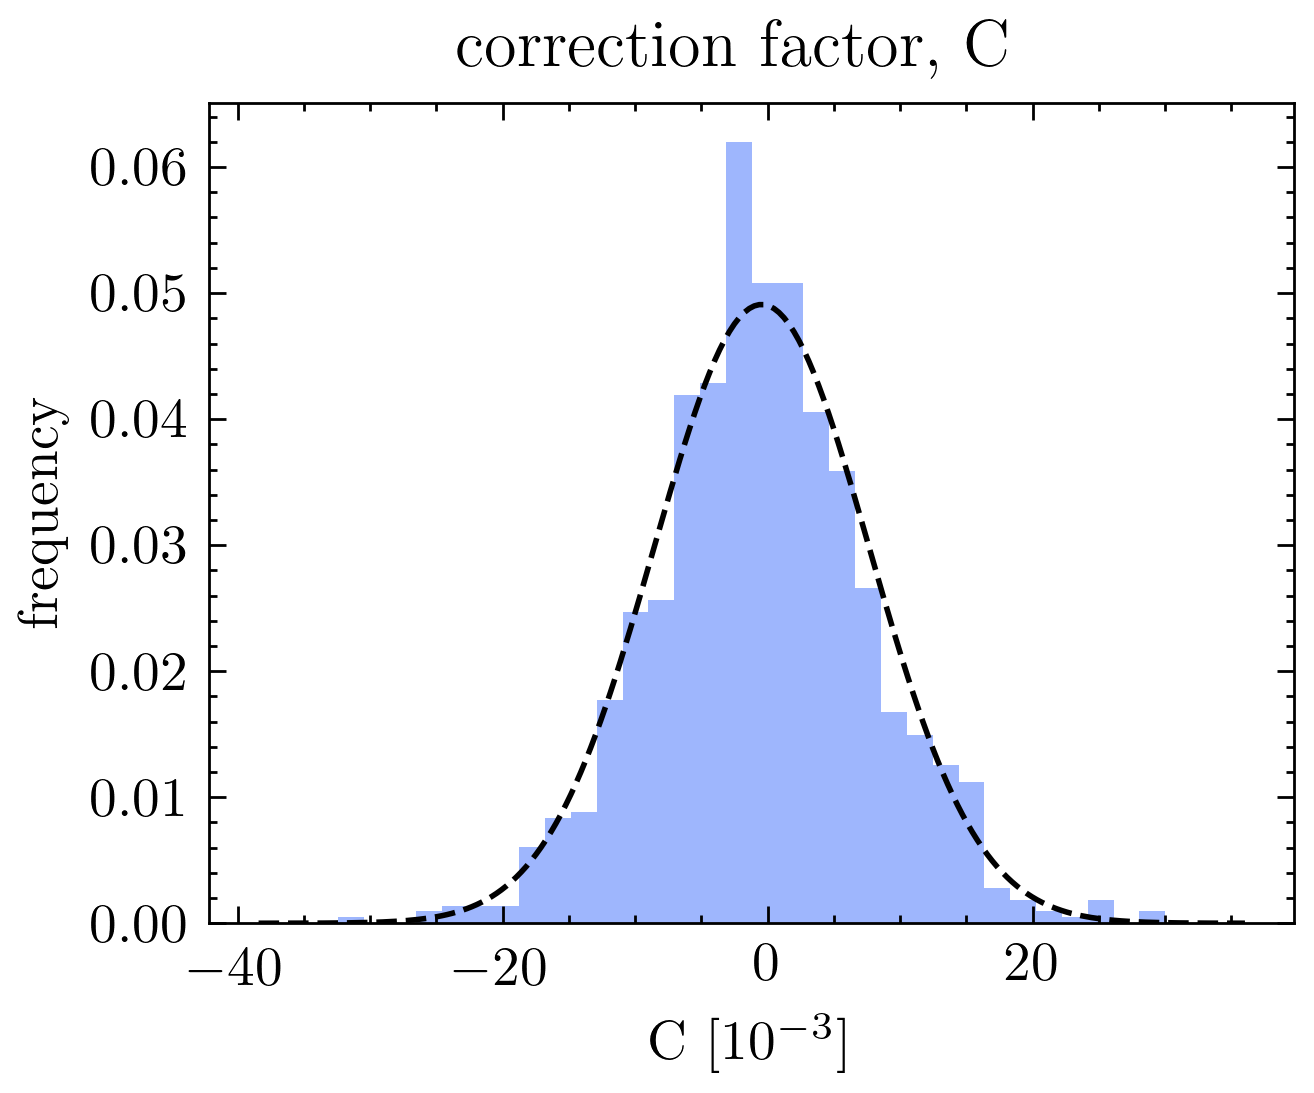
\includegraphics[width=0.4\textwidth]{figures/chap3/C_factor_hist.png}
		\label{fig:C_factor_hist}}
	
	\caption{The linear correction factor $C(\tau,E)$, from \cref{eqn:deltaA_linear_correction}.}
	\label{fig:C_factor}
	% datasets: ???
	% python script: ???
\end{figure}

\begin{figure}
	\centering
	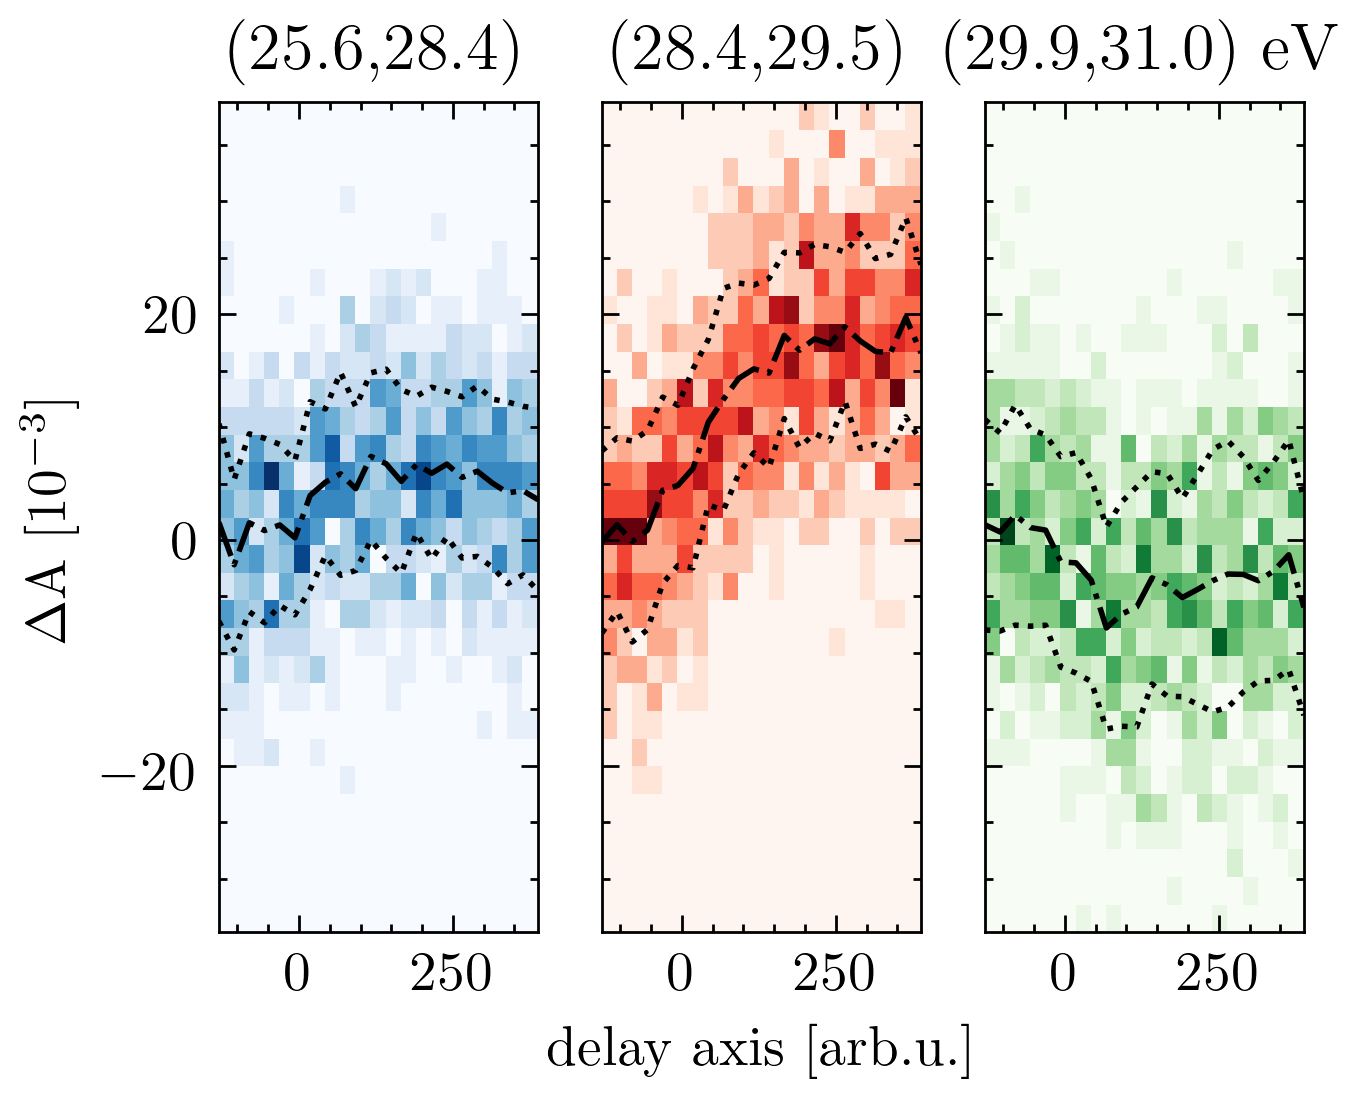
\includegraphics[width=0.5\textwidth]{figures/chap3/corrected_hist.png}
	\caption{histogram of spectral features from dataset with correction factor $C(\tau,E)$ applied }
	\label{fig:corrected_hist}
	% data set: ???
	% figure made using: ???
\end{figure}

\begin{figure}
	\centering
	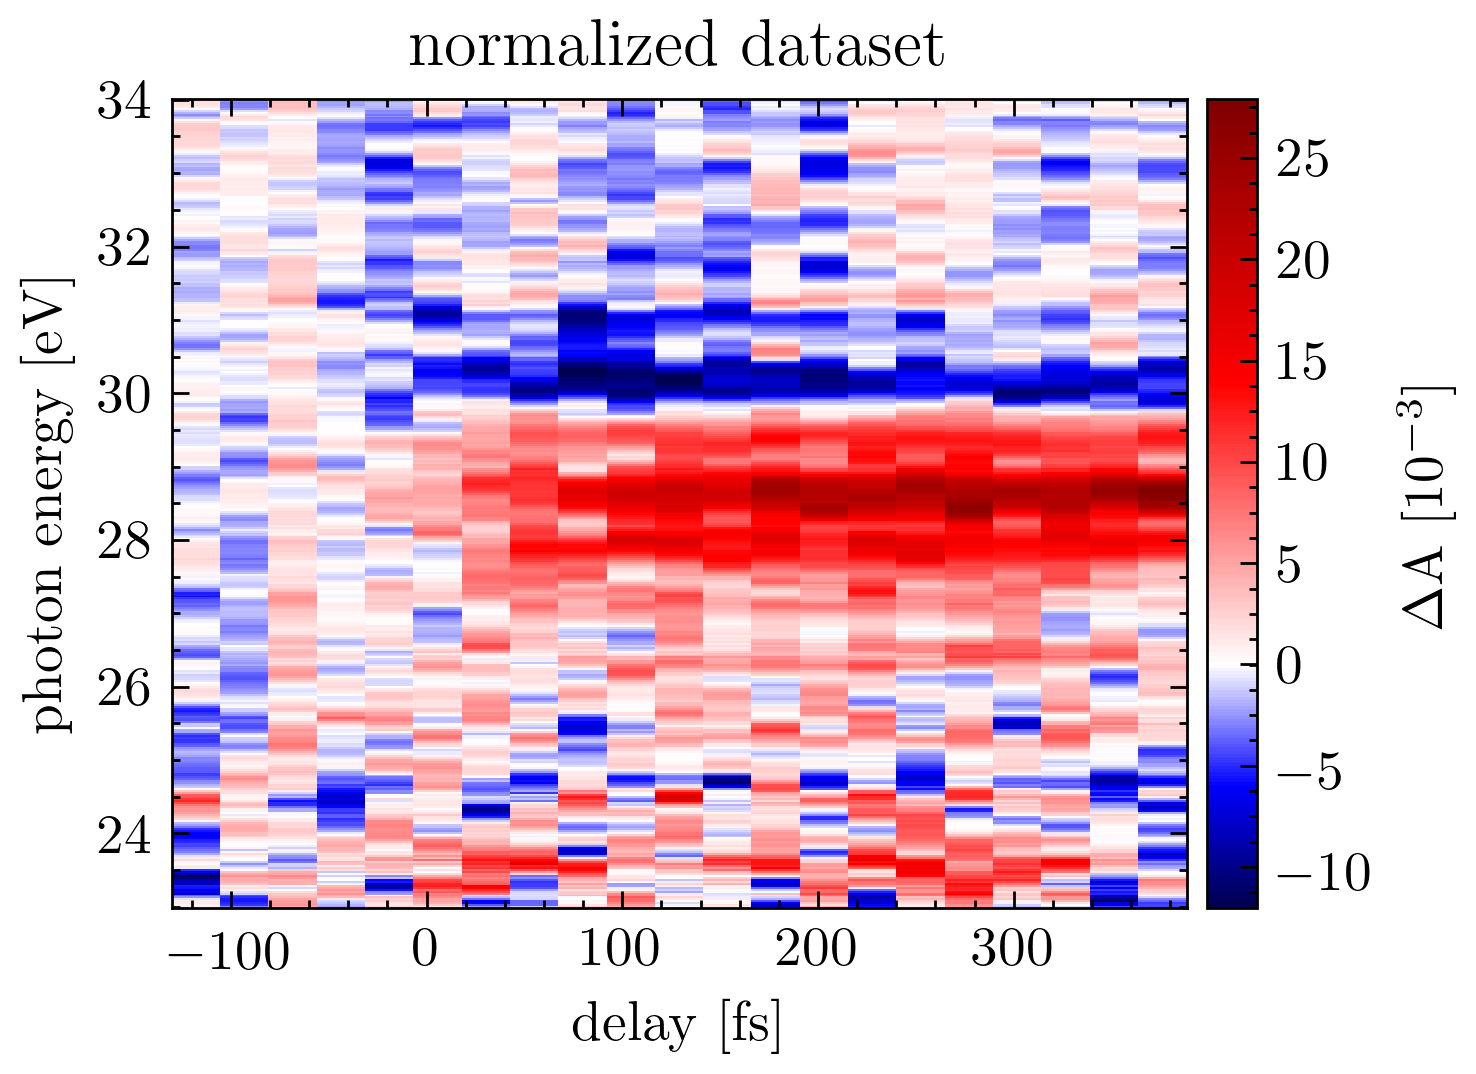
\includegraphics[width=0.5\textwidth]{figures/chap3/Ge_corrected_raw_spectrogram.png}
	\caption{normalized dataset: dataset with correction factor $C(\tau,E)$ applied }
	\label{fig:Ge_corrected_raw_spectrogram}
	% data set: ???
	% figure made using: ???
\end{figure}

\begin{figure}
	\centering
	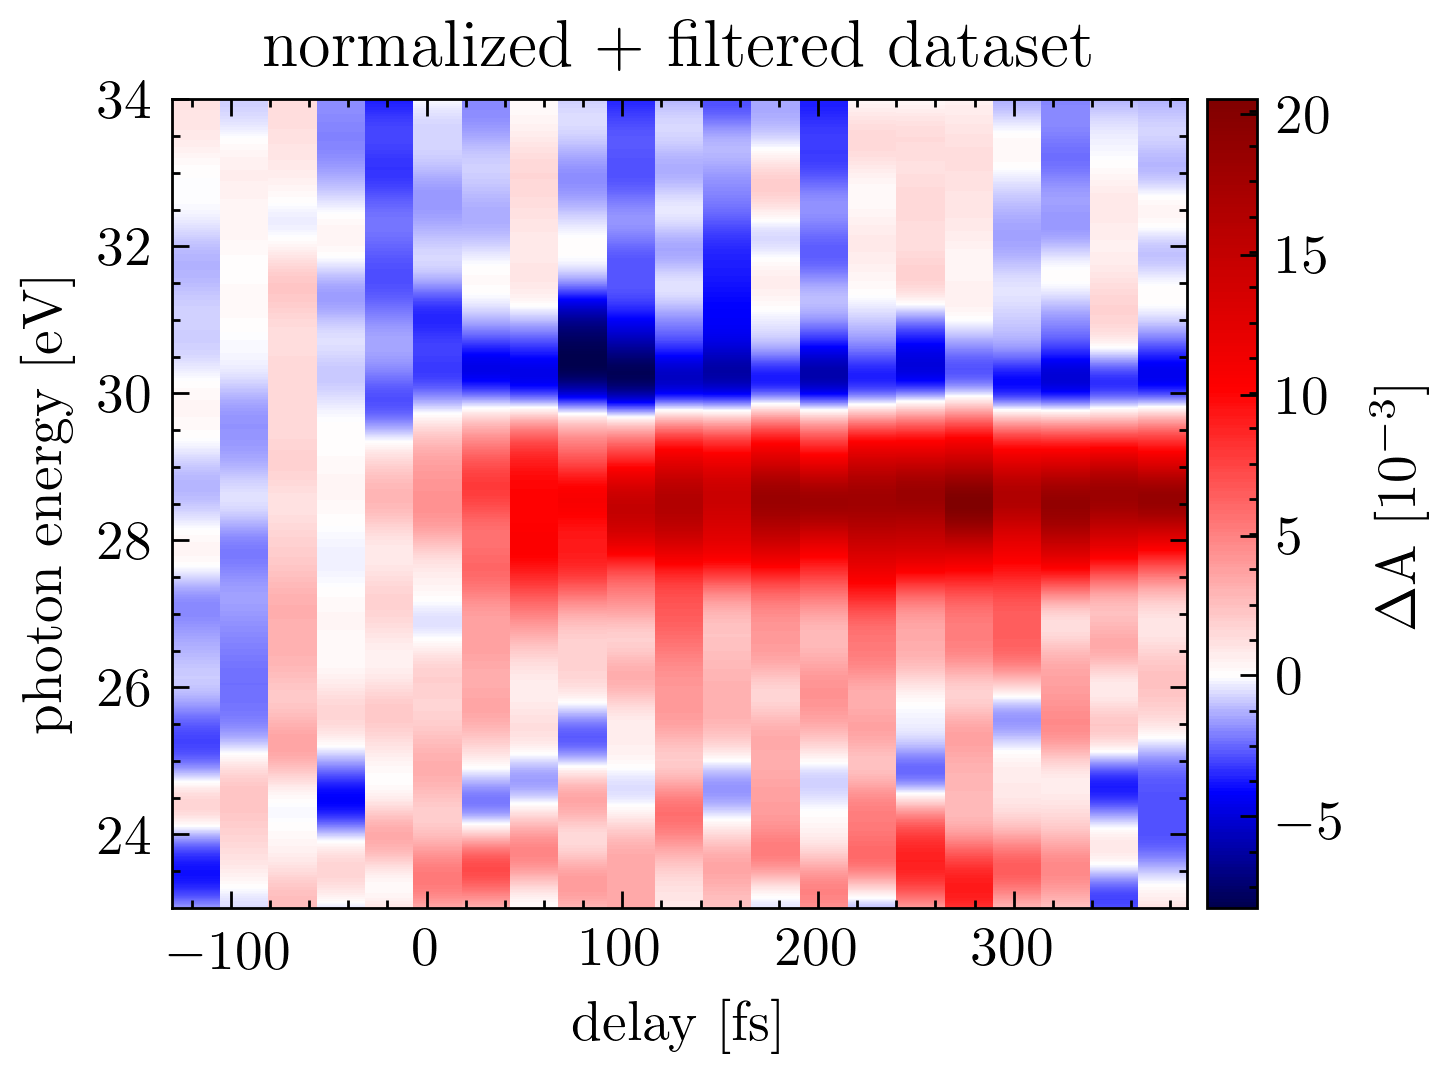
\includegraphics[width=0.5\textwidth]{figures/chap3/Ge_corrected_filtered_spectrogram.png}
	\caption{normalized dataset with frequency filter applied }
	\label{fig:Ge_corrected_filtered_spectrogram}
	% data set: ???
	% figure made using: ???
\end{figure}

In this section we will describe the procedure used to analyze the data, starting with the raw data files from the CMOS camera.

\begin{enumerate}
	\item calibration of spectrometer energy axis and delay axis (just state it as fact, don't go into detail)
	\item data reduction: 2D image to 1D spectral lineout for each measurement. note that the jacobian needs to be used for plotting counts vs energy, but not for $\Delta A$ or $A$ since it divides out
	\item investigation of noise: peaks vs valleys vs slopes of harmonics. most of the noise comes from not the peaks, so we use the value at the peak for later analysis
	\item sample drilling or harmonic drift? inconclusive? or \textit{no conclusive evidence of drilling?}
	\item correlations between different harmonic peaks in $\Delta A$
	\item linear correction method $C(\tau,E)$
	\item choice of dx=2 method
	\item frequency filtering
	\item failed methods: SVD, interpolation
\end{enumerate}

The XUV photon spectrometer utilizes a flat field grating (Hitachi, 1200 l/mm) to spectrally disperse the XUV light onto the detector. The grating is designed to focus along the spectral axis (horizontal direction of sensor) while preserving the spatial profile of the beam (vertical direction). The focus of the grating is incident on a 75 mm diameter imaging quality microchannel plate (MCP) array (Photonis), which converts the XUV photons into electrons via a nonlinear avalanche process with a gain of approximately $10^6 - 10^8$. These electrons are accelerated towards a phosphor screen, which converts the electrons into visible photons with a central wavelength of $\sim480$ nm. The visible photons exit the vacuum chamber via a glass feedthrough and are imaged by a lens onto a CMOS sensor of a digital camera (Andor). The recorded data is a two dimensional array of counts, with the horizontal axis representing the spectral content and the vertical axis representing the spatial profile of the beam.

talk about all the steps you use to process the data, starting from the 2d image and ending with the delta-A spectrogram.

\subsection{energy and delay calibration}
\subsection{A note about the Jacobian}

At each pixel, the spectrometer's camera records the integrated counts within the area of one pixel. We wish to convert the measured dataset (counts \textit{vs.} spectral pixel) to a physically meaningful spectrum (counts \textit{vs.} photon energy) while conserving energy \cite{mooneyGetBasicsRight2013}.

More precisely, our measurement samples a counts function $f_p$ in the spectral pixel basis $p$:
\begin{equation}
f_p (p): \text{spectral pixel} \rightarrow \text{counts}.
\end{equation}
The spectral pixel value is proportional to wavelength, with some extra factors that account for the geometry of the detector relative to the grating. We can convert the domain of the spectrometer's dataset from spectral pixels $p$ to energy $E$ (in eV) using an invertible polynomial transformation\footnote{The details surrounding the choice of this transformation will be discussed elsewhere in the dissertation.}:
\begin{equation}
\begin{aligned}
E(p)&: \text{spectral pixel} \rightarrow \text{energy [eV]}, \\
E(p) &= a_4 p^2 + a_3 p^3 + a_2 p^2 + a_1 p + a_0.
\end{aligned}
\end{equation}
Let the inverse of $E(p)$ be $p(E)$. From energy conservation, the transformation must preserve the integrated counts:
\begin{equation}
f_p(p) \text{ } dp = f_E(E) \text{ } dE.
\end{equation}
Rearranging, we obtain an expression for the counts expressed in the energy domain, $f_E$:
\begin{equation}
f_E (E) = f_p (p) \frac{dp}{dE} = f_p(p) \frac{d}{dE} p(E).
\label{eqn:spectrometer_jacobian}
\end{equation}
Therfore, the measured spectrum $f_p(p)$ in the pixel basis can be converted to the energy basis by multiplying it by a factor of $\frac{d}{dE} p(E)$. Note that this factor is only important when considering spectrometer counts; calculations of $A$ or $\Delta A$ can omit the Jacobian as it is common to both spectra and will divide out.

\subsection{source of noise}
\subsection{sample drilling or random drift?}
\subsection{correlations between harmonic peaks in $\Delta A$}
\subsection{integration vs summation near harmonic peaks}
\subsection{apparent $\omega$ and $2\omega$ oscillations in data}



mention calibration of spectrometer in passing, 2D image $\rightarrow$ 1D spectrum. jacobian needs to be used for plotting counts vs energy, but not for delta-OD, OD or transmission figures.

\begin{equation}
\Delta A^{\text{meas}}(\tau, E) = -\log_{10} \left( \frac{I_{on} f}{I_{off}} \right) = \Delta A^{\text{norm}}(\tau,E) + C(\tau,E)
\label{eqn:deltaA_linear_correction}
\end{equation}
